\subsubsection{Optimization in a Box}
We have $N = 40$ and $n = 30$. We choose the ODE tolerance to be $10^{-7}$ and the optimization tolerance is $10^{-3}$. We choose $\bar \rho = 0.036$.
We set up a test problem which sets $\hr$ to be the forward solution for the problem with $V_{ext} = cy$, where $c = 0.1$, as in Archer's paper. The optimization forward problem is such that $c = 0.01$ and $\w = \mathbf 0$. We expect the control to act downward, since the strength of gravity $c$ is decreased.
We also expect that the cost $\mathcal J$ is decreasing from the baseline $J_{FW}$ when optimizing.
For $\beta = 10^{-3}$ and $\beta = 10^{-1}$ this works well.
When $\beta = 10^{-3}$ we get $J_{FW} = 0.4955$ and $J_{Opt} = 0.0556 $. 
The results can be seen in Figures \ref{Fa1}, \ref{Fa2} and \ref{Fa3}.
\begin{figure}[h]
	\centering
	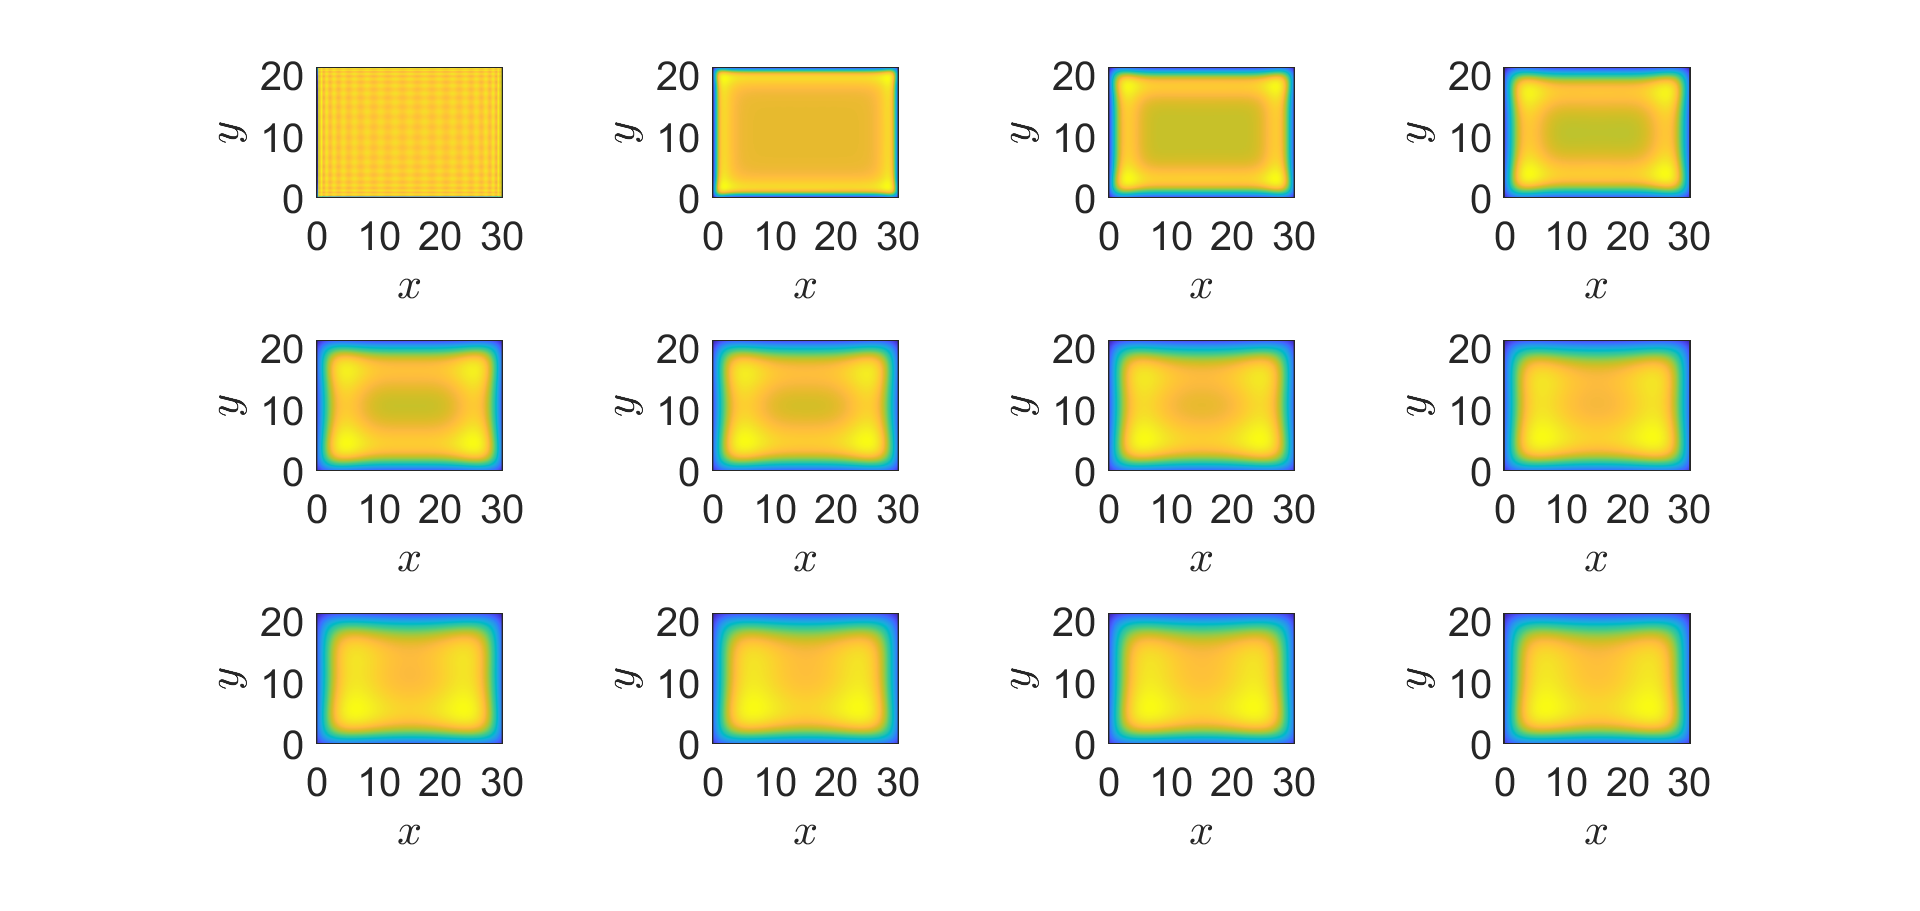
\includegraphics[scale=0.35]{F11.png}
	\caption{Forward $\rho$ for $c = 0.01$} 
	\label{Fa1}
\end{figure}	
\begin{figure}[h]
	\centering
	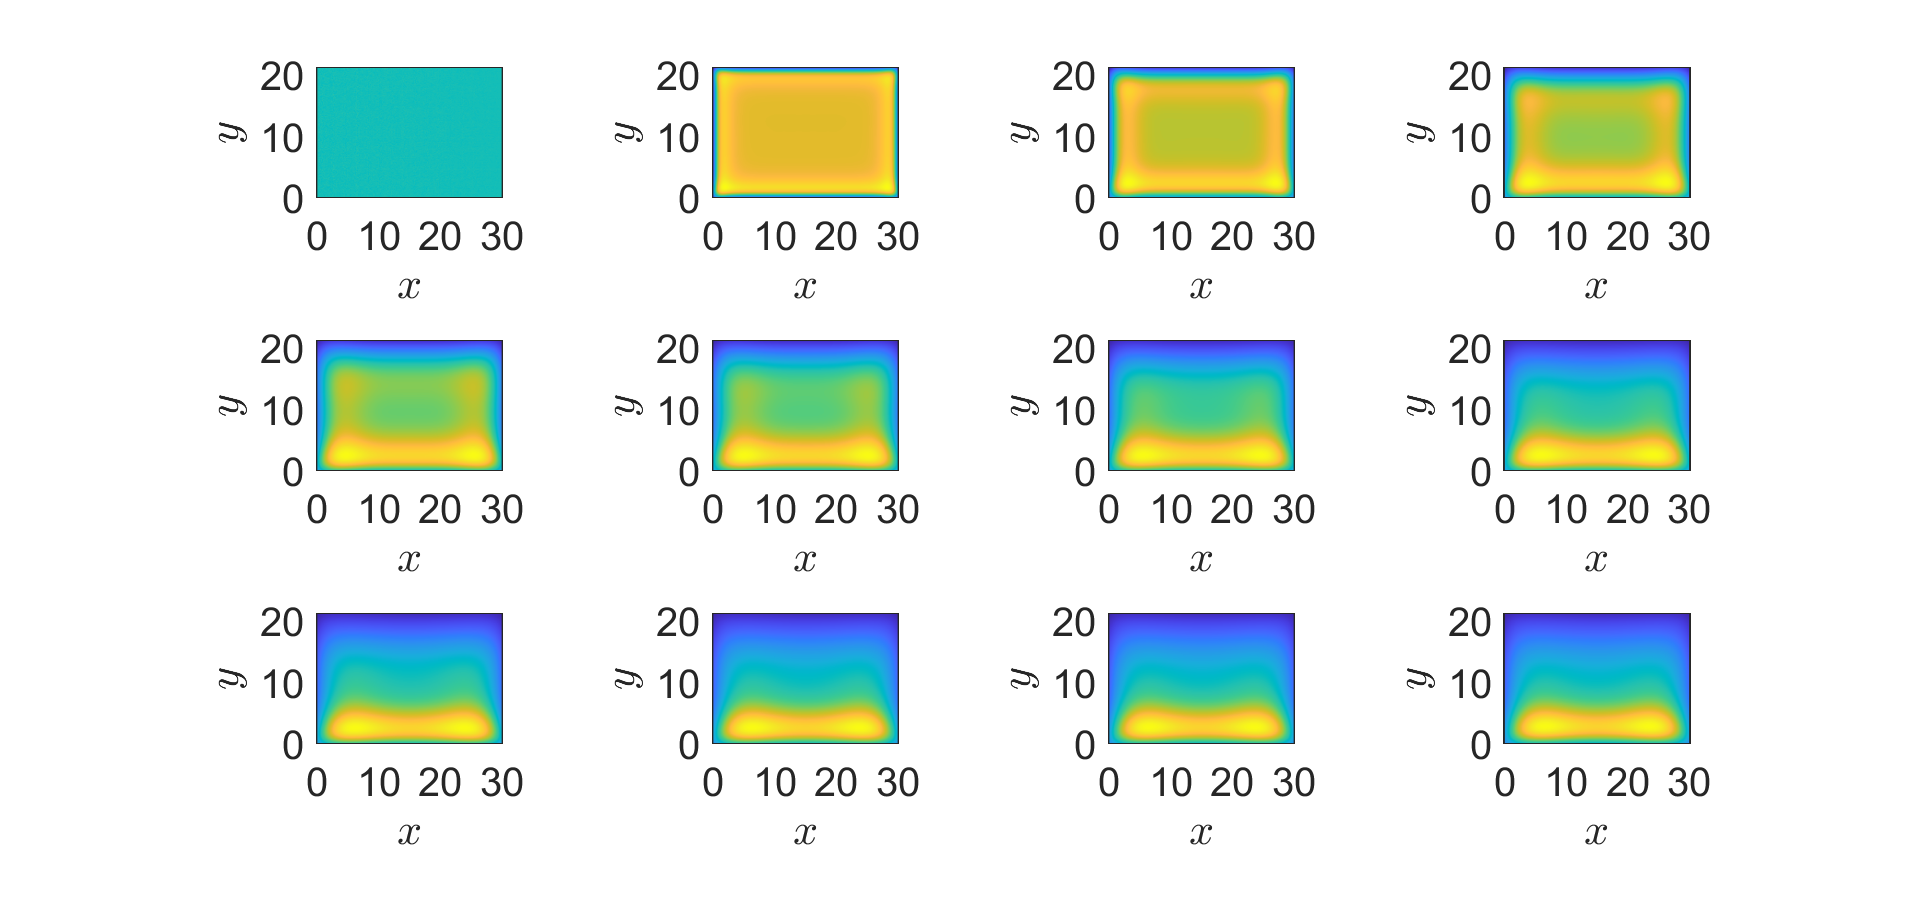
\includegraphics[scale=0.35]{F21.png}
	\caption{Optimal $\rho$ for $c = 0.01$} 
	\label{Fa2}
\end{figure}
\begin{figure}[h]
	\centering
	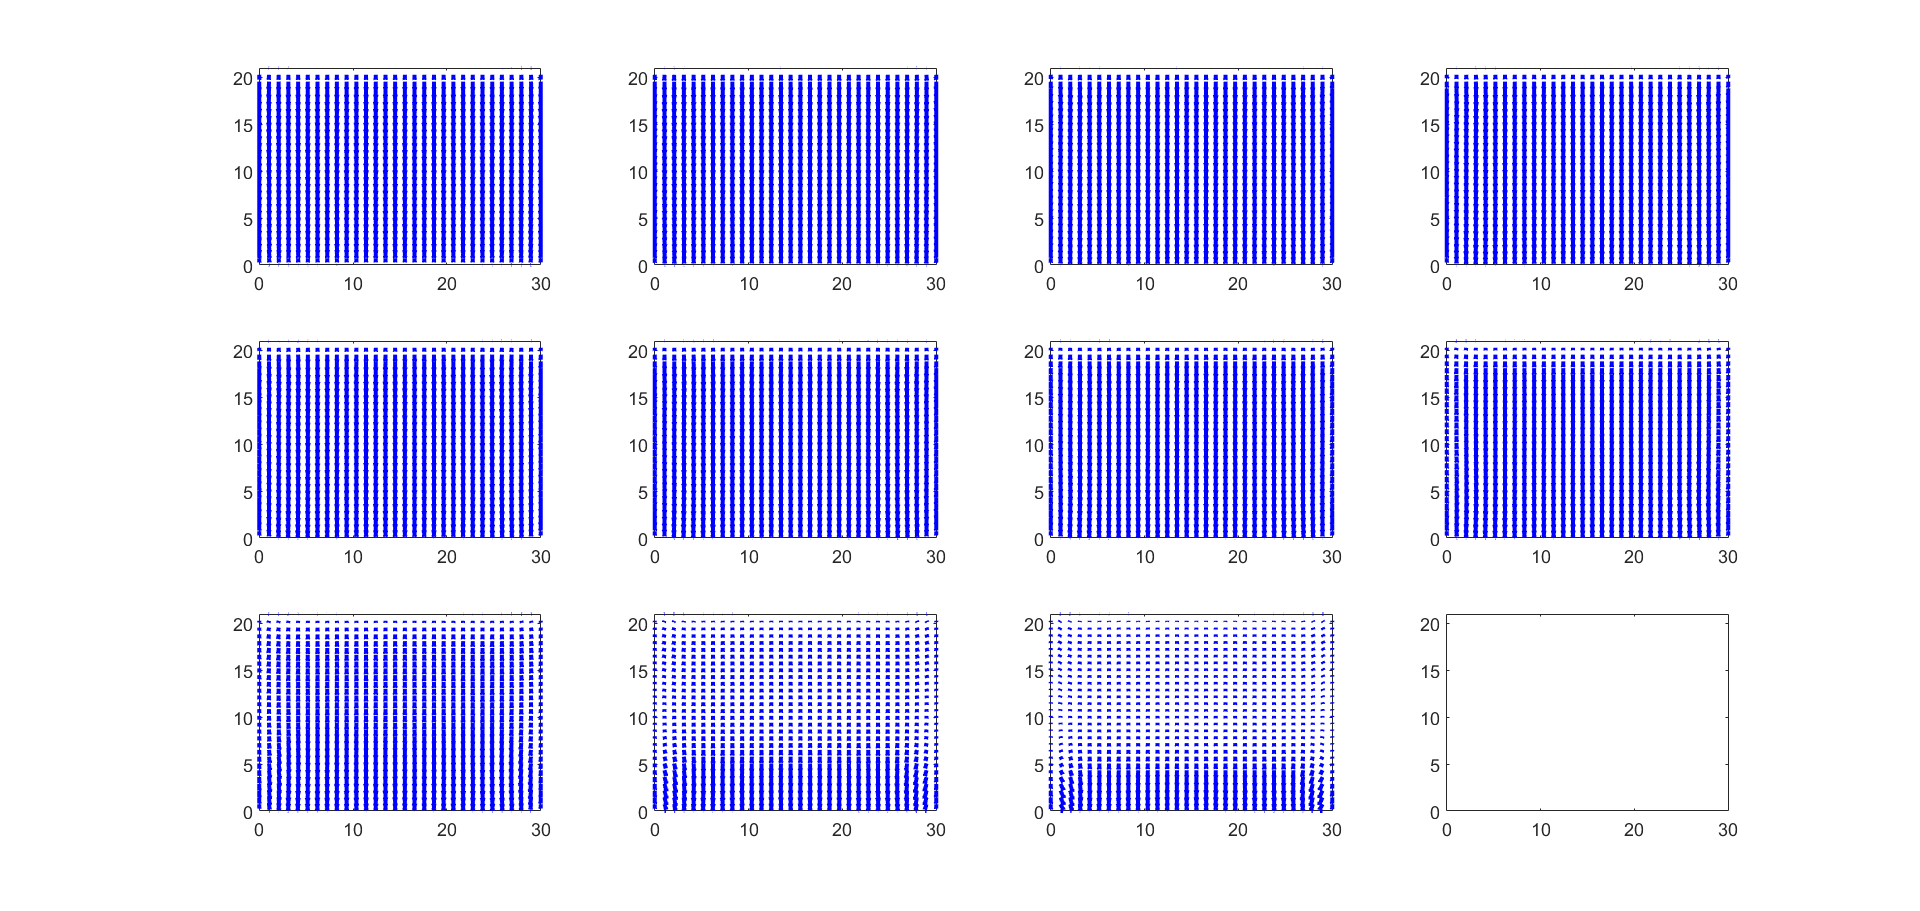
\includegraphics[scale=0.35]{F31.png}
	\caption{Optimal Control for $c = 0.01$} 
	\label{Fa3}
\end{figure}



\subsubsection{Optimization in a Box - Time-Independent Control}
We consider the identical problem but now require the control to be time independent. This affects the gradient equation as discussed in Section \ref{sec:TimeIndependentControl}.
Therefore, we expect a $\w$ which is averaged over the time horizon and therefore time independent. The result is $J_{FW} = 0.4855$ and $J_{Opt} = 0.0733$ and can be seen in Figures \ref{F6a}, \ref{F7a} and \ref{F8a}. We observe that, as expected, $J_{opt}$ is larger than for the previous example where $\w$ was allowed to vary over time.

\begin{figure}[h]
	\centering
	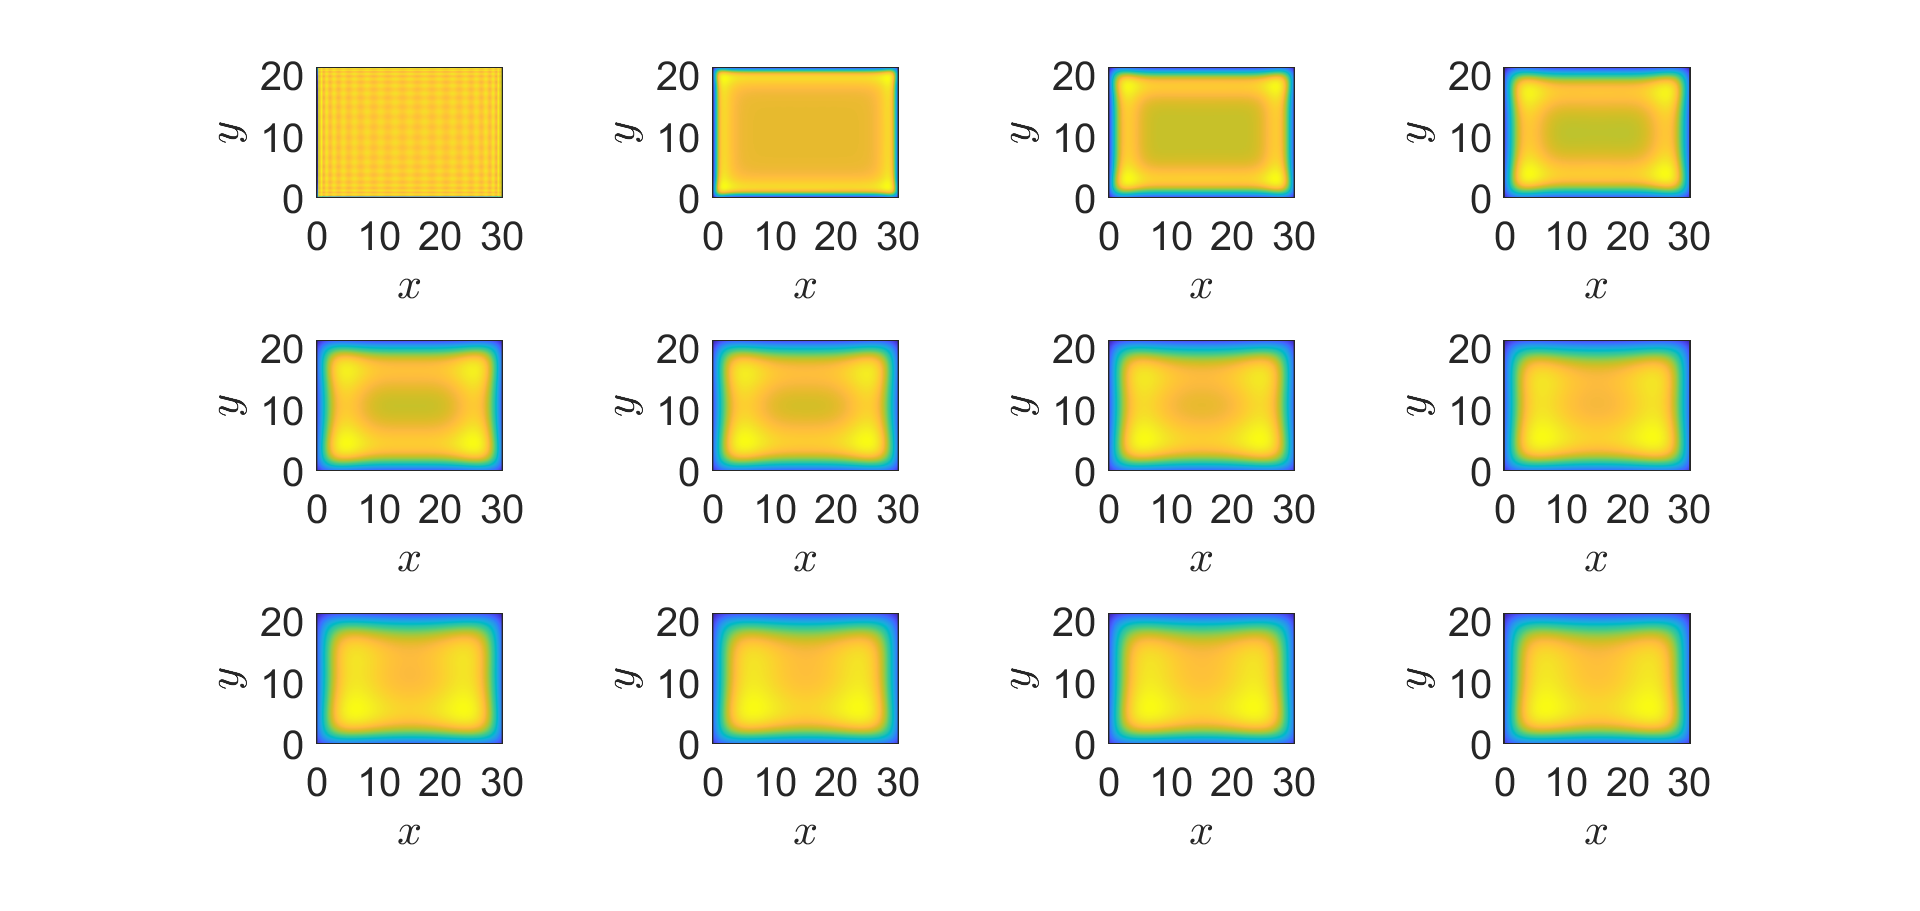
\includegraphics[scale=0.35]{C1.png}
	\caption{Time-independent; Forward $\rho$ for $a = 0.01$} 
	\label{F6a}
\end{figure}	
\begin{figure}[h]
	\centering
	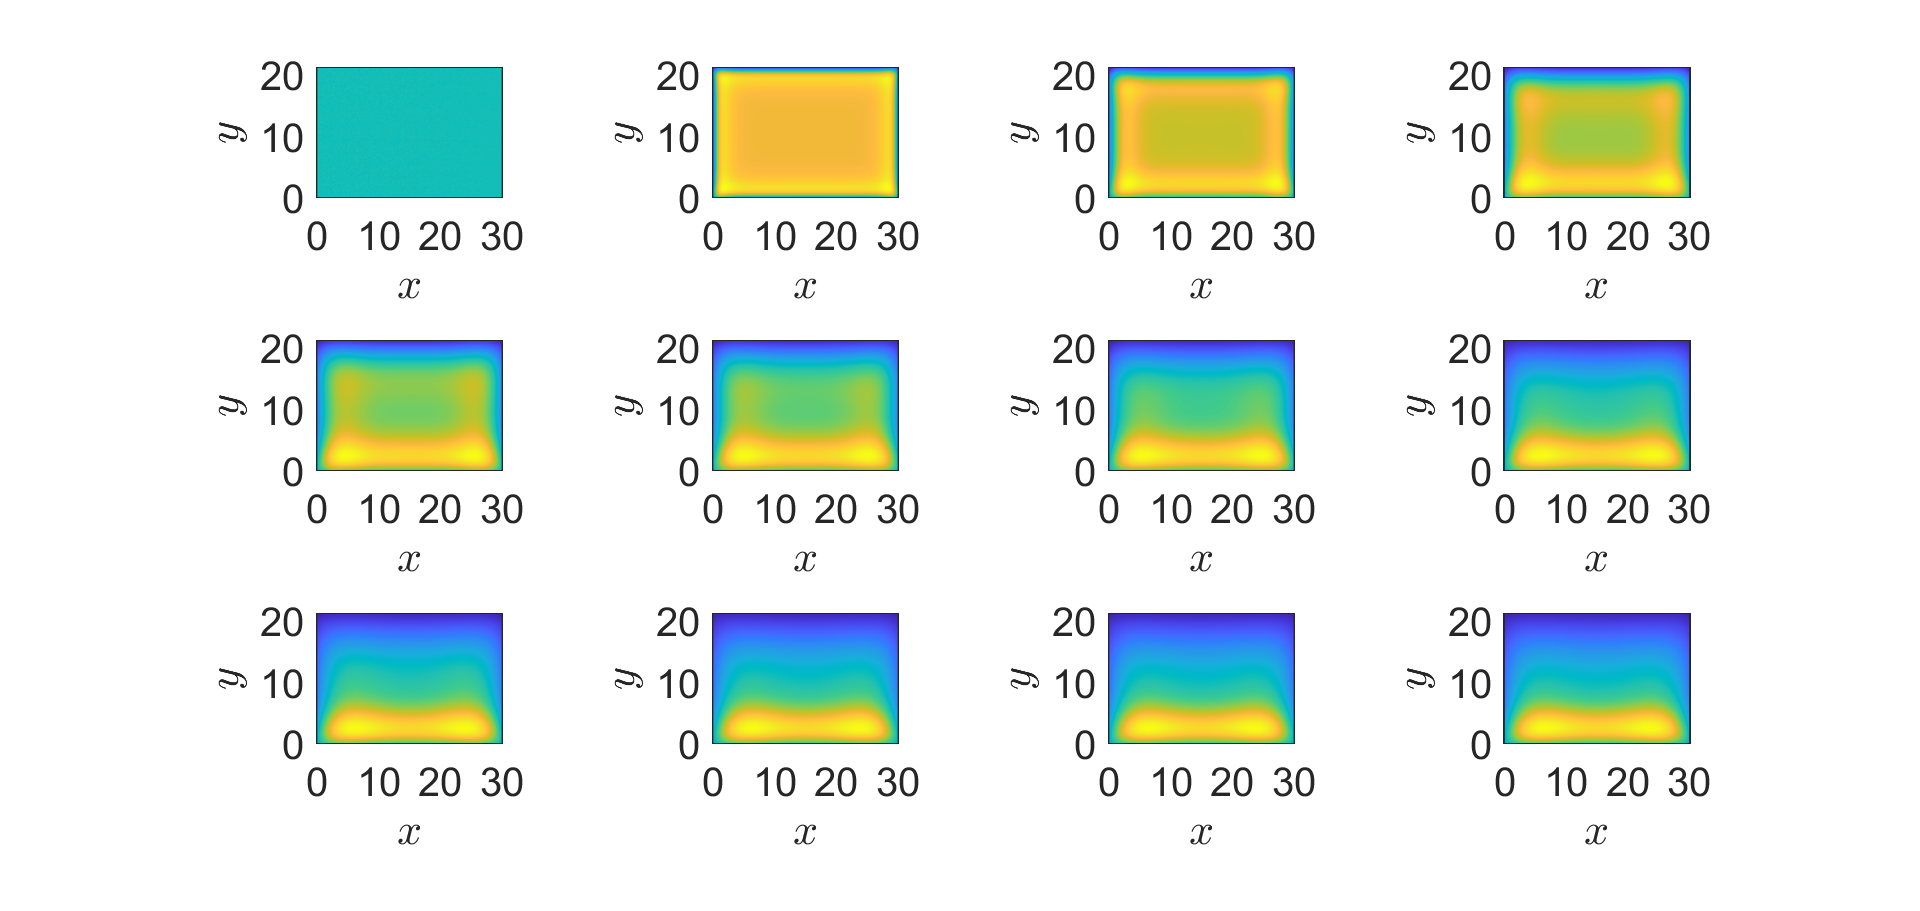
\includegraphics[scale=0.35]{C2.png}
	\caption{Time-independent; Optimal $\rho$ for $a = 0.01$} 
	\label{F7a}
\end{figure}
\begin{figure}[h]
	\centering
	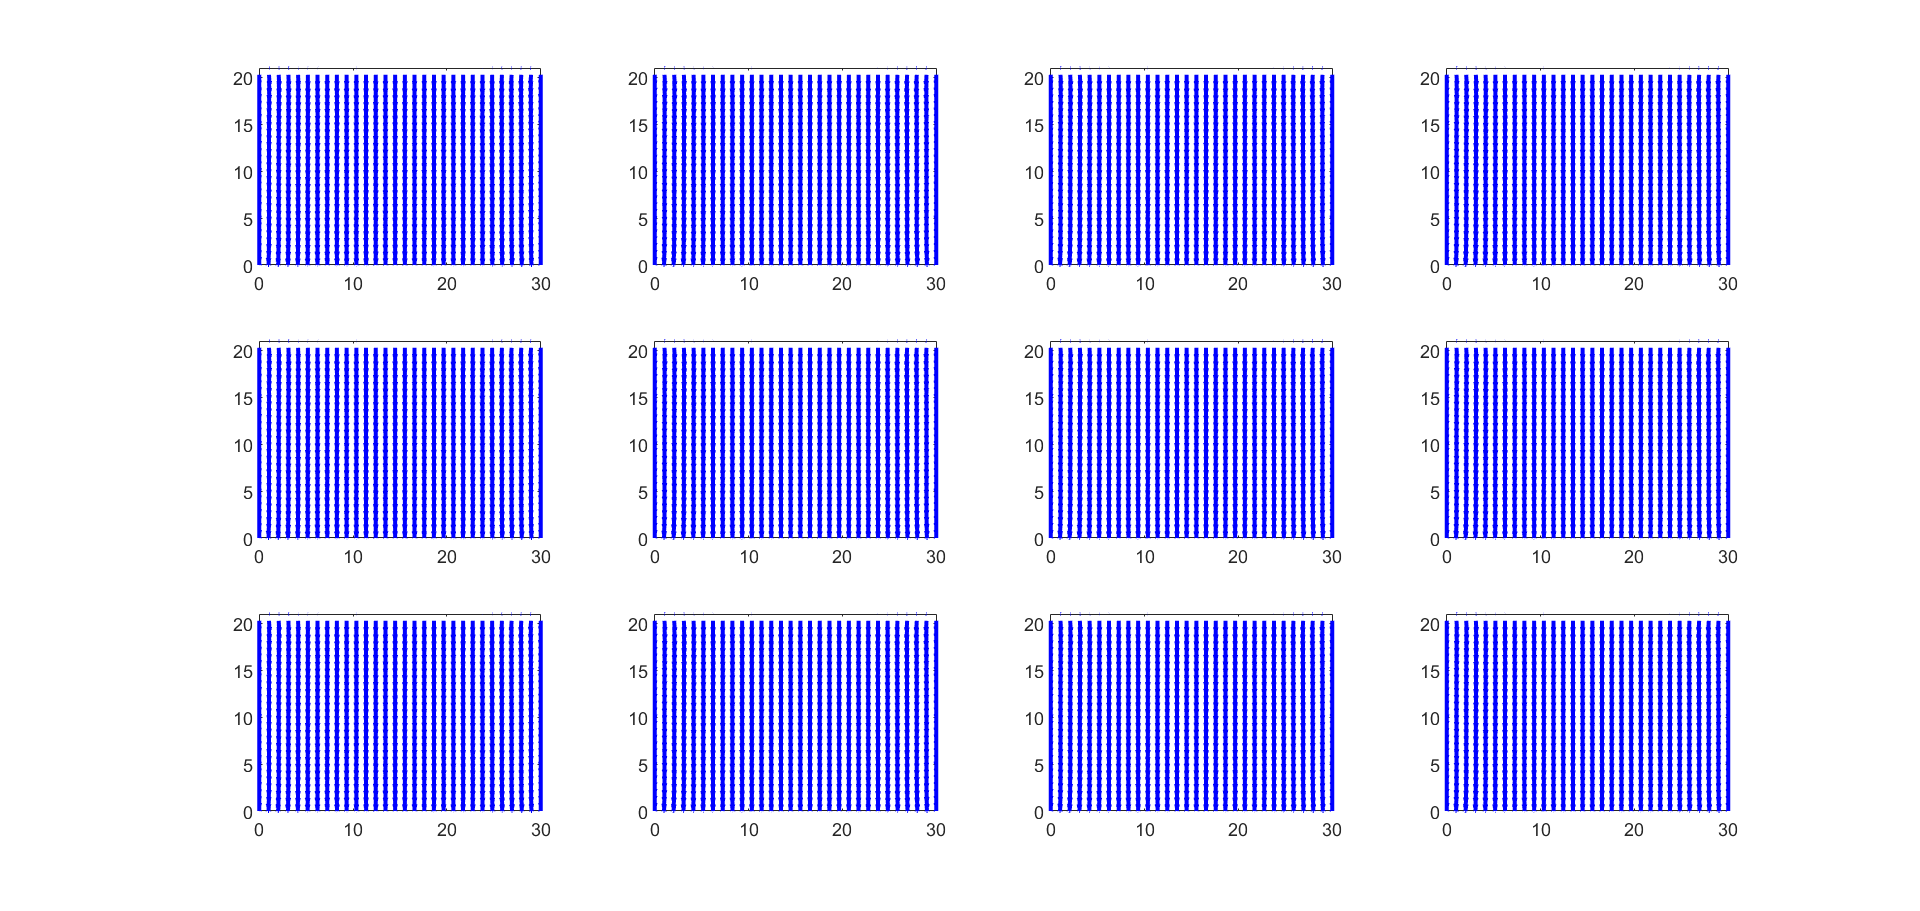
\includegraphics[scale=0.35]{C3.png}
	\caption{Time-independent; Optimal Control for $a = 0.01$} 
	\label{F8a}
\end{figure}

We wanted to see whether the time independent flow control is similar to the $\nabla V_{ext}$ of the target.
The target state was influenced by $V_{ext} = 0.1 y_2$. The forward state for the OCP was influenced by $V_{ext} = 0.01 y_2$. 
Figure \ref{F1a} shows the control and $\nabla V_{ext}$ of the target. We can see that one of these is positive, while the other one is negative. This is due to the opposite signs of $\w$ and $\nabla V_{ext}$ in the PDE.

\begin{figure}[h]
	\centering
	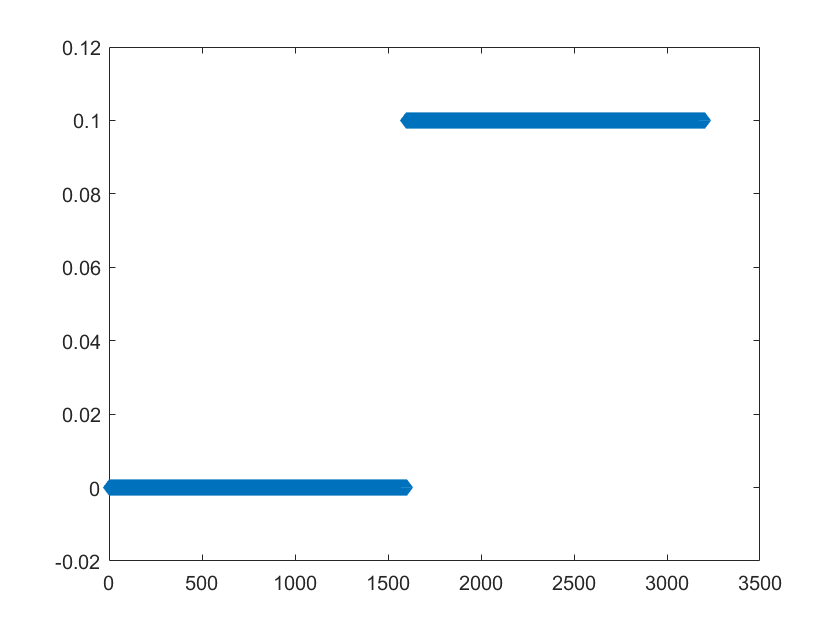
\includegraphics[scale=0.35]{V1.png}
	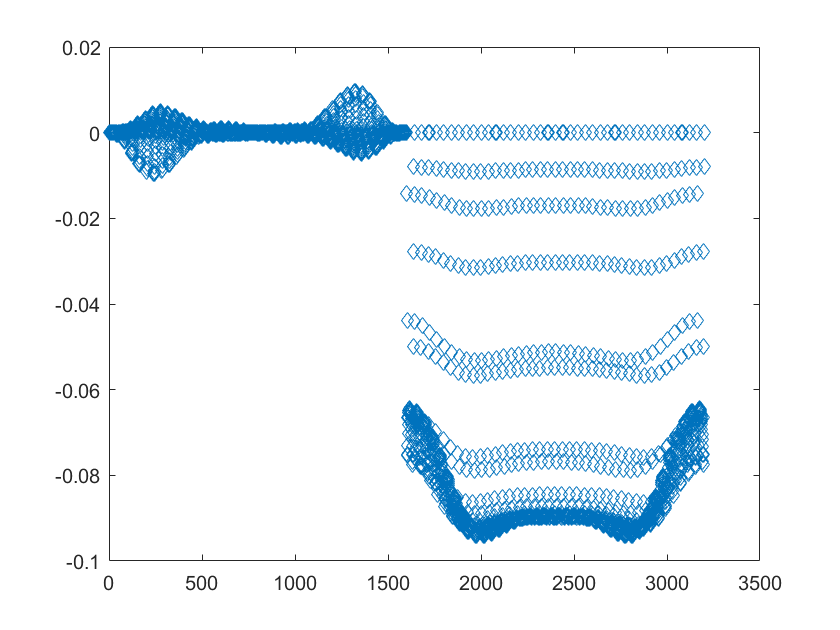
\includegraphics[scale=0.35]{W1.png}
	\caption{$\nabla V_{ext}$ of target and optimal control $\w$.} 
	\label{F1a}
\end{figure}

\subsubsection{Optimization in a Periodic Box}

\subsubsection{Optimization in a Periodic Box - Time-Independent Control}

\subsubsection{Optimization in a Multishape}
The first example is a simple mulitshape with two quadrilaterals. We choose $n = 30$ and $N = 20$ and run up to time $T = 30$, the parameter choices are as in the section on optimization in a box. We choose $\lambda = 0.01$ as usual. We get $J_{FW} = 0.0713$ and $J_{Opt} = 0.0059$. The results are displayed in Figures \ref{FM0} and \ref{FM0a}.
\begin{figure}[h]
	\centering
	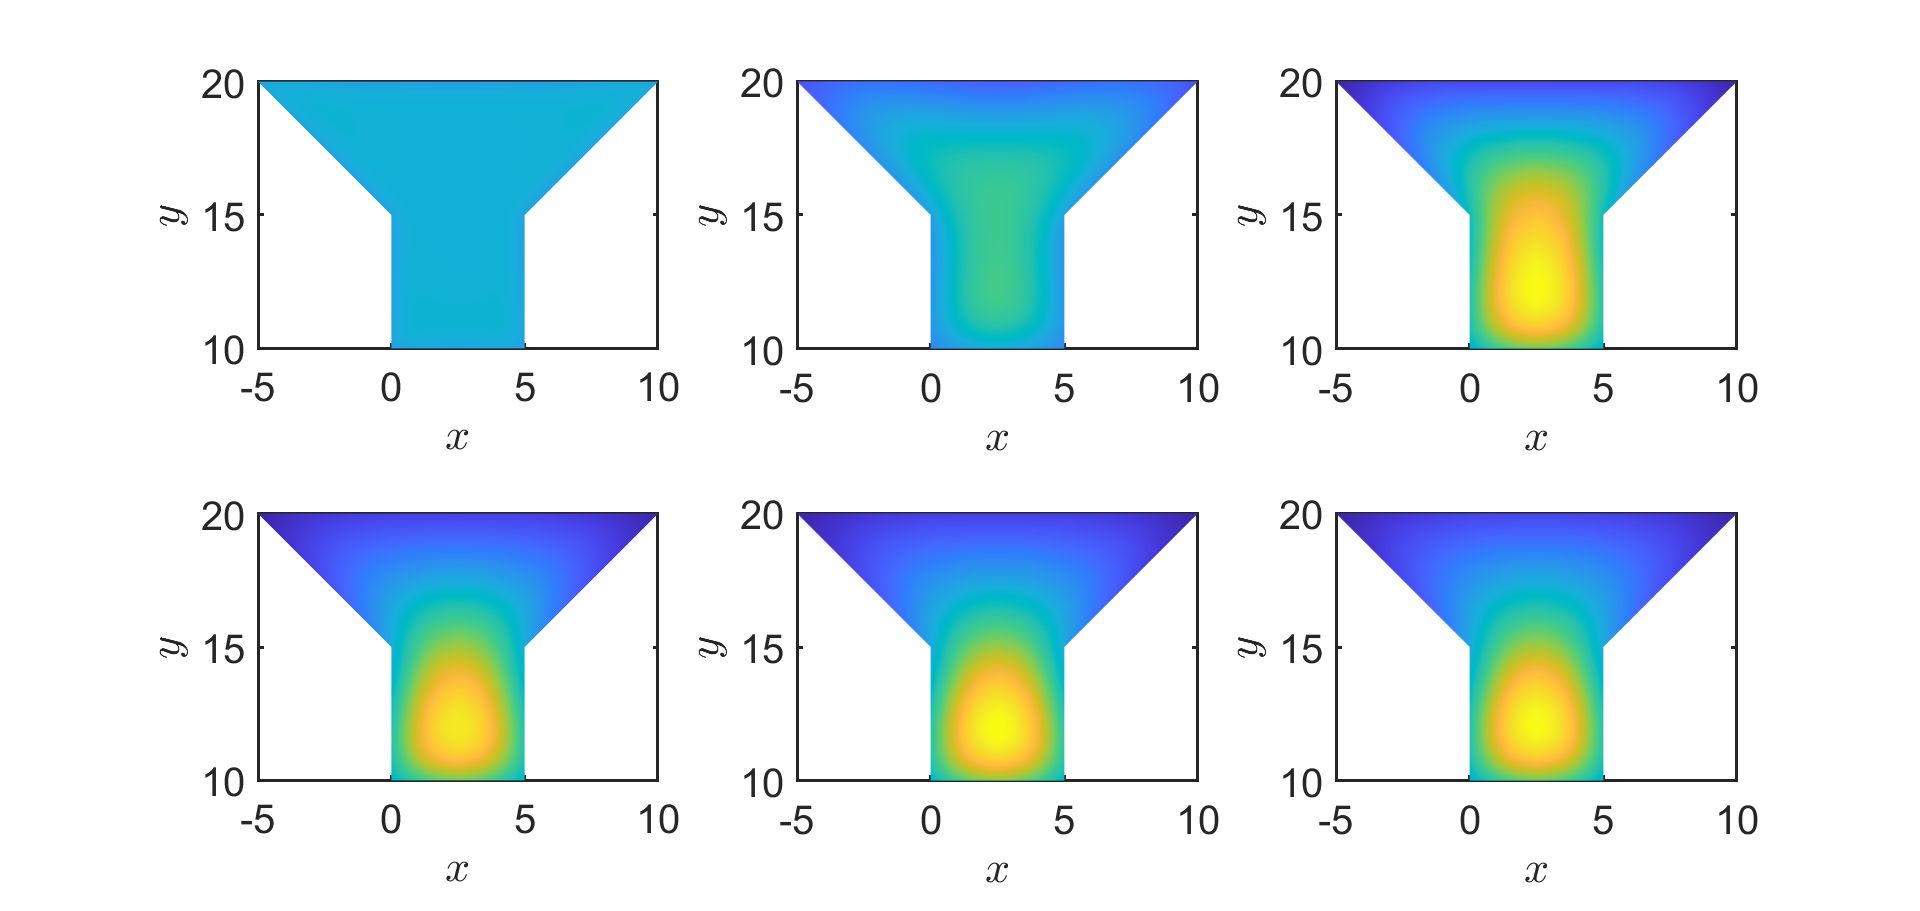
\includegraphics[scale=0.35]{MultiOpt1a.png}
	\caption{Multishape Example 1: Optimal $\rho$} 
	\label{FM0}
\end{figure}
\begin{figure}[h]
	\centering
	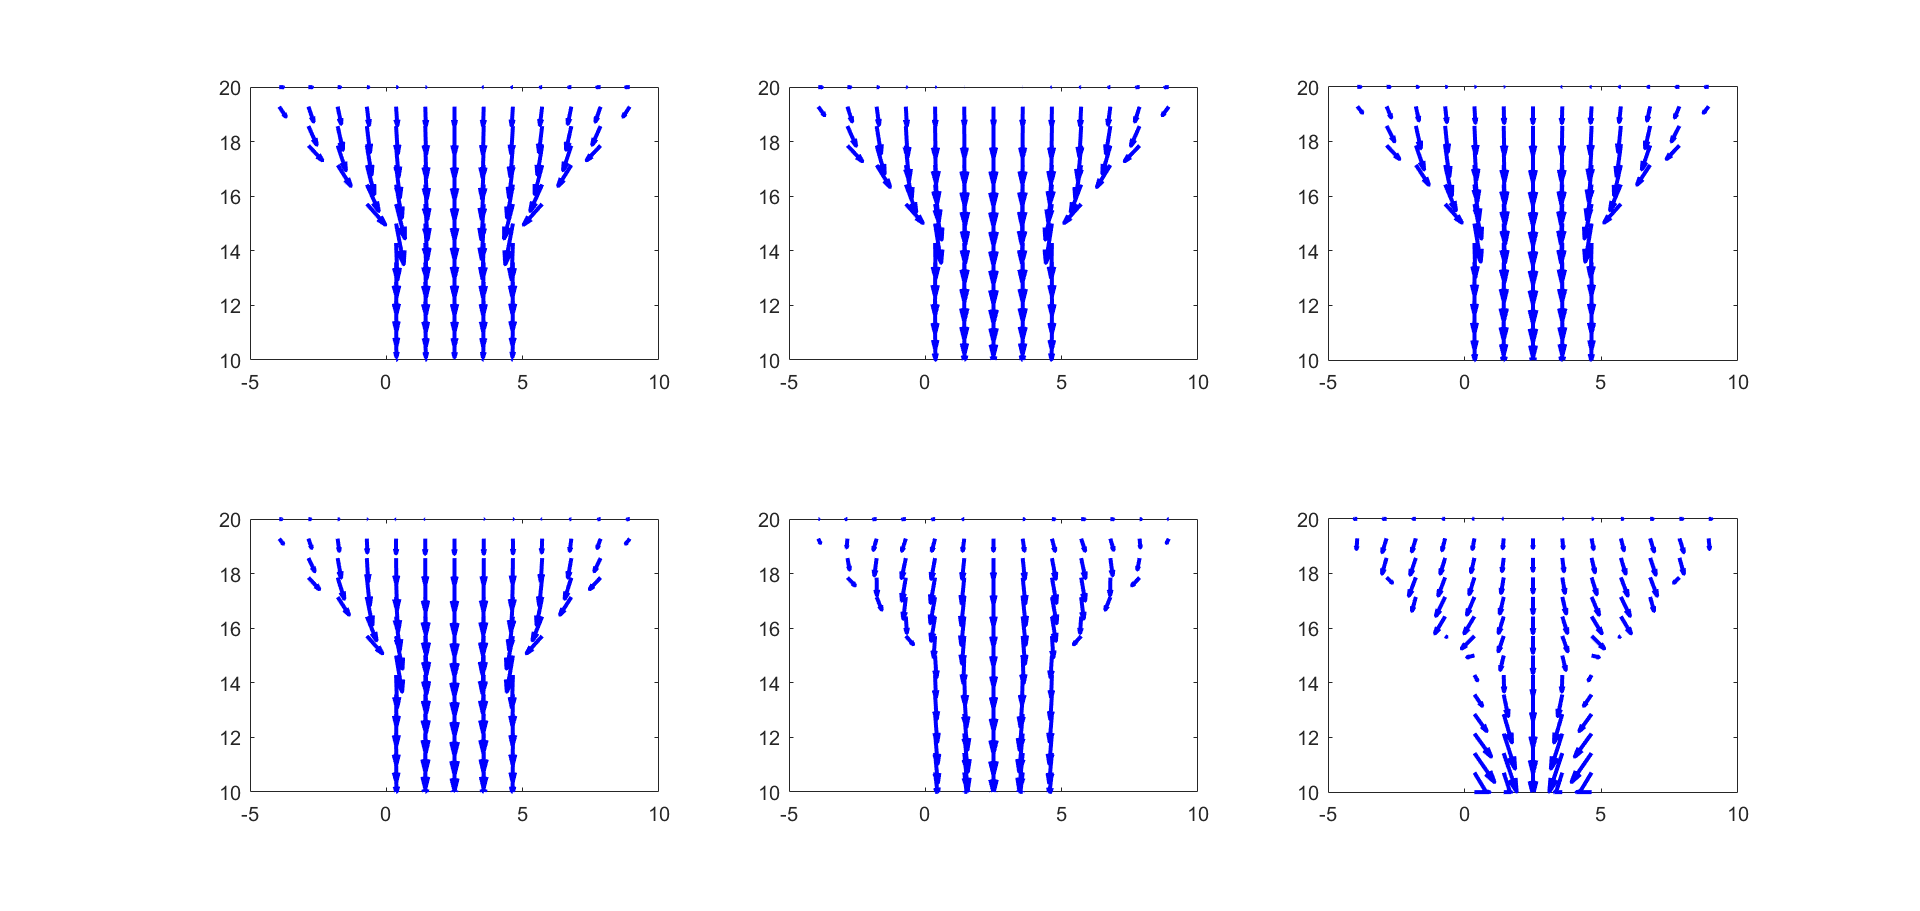
\includegraphics[scale=0.35]{MultiCont1a.png}
	\caption{Multishape Example 1: Optimal control} 
	\label{FM0a}
\end{figure}
\\
\\
The second example is an optimization problem in a larger multishape. The setup remains the same as before, but now computed on a multishape which is comprised of four shapes, out of which three are quadrilaterals and one is a wedge. We get $J_{FW} = 0.0766$ and $J_{Opt} = 0.0116$. The results can be seen in Figures \ref{FM1a} and \ref{FM2a}.
\begin{figure}[h]
	\centering
	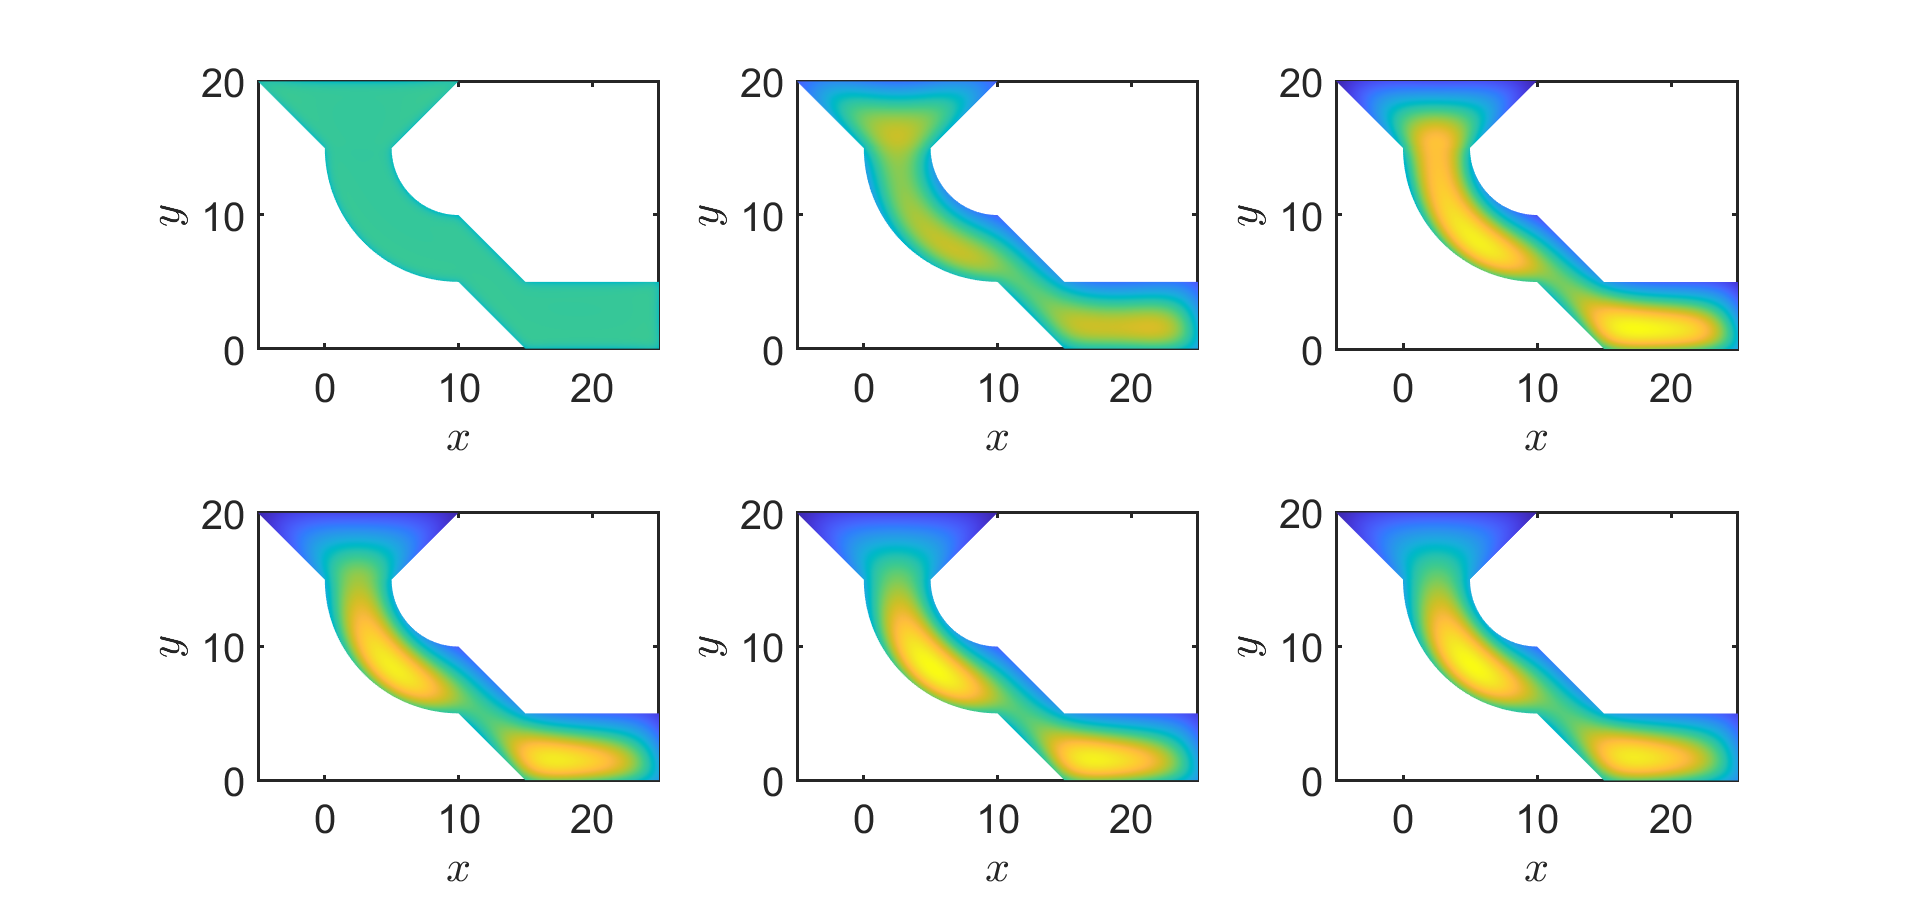
\includegraphics[scale=0.35]{MultiOpt2.png}
	\caption{Multishape Example 2: Optimal $\rho$} 
	\label{FM1a}
\end{figure}
\begin{figure}[h]
	\centering
	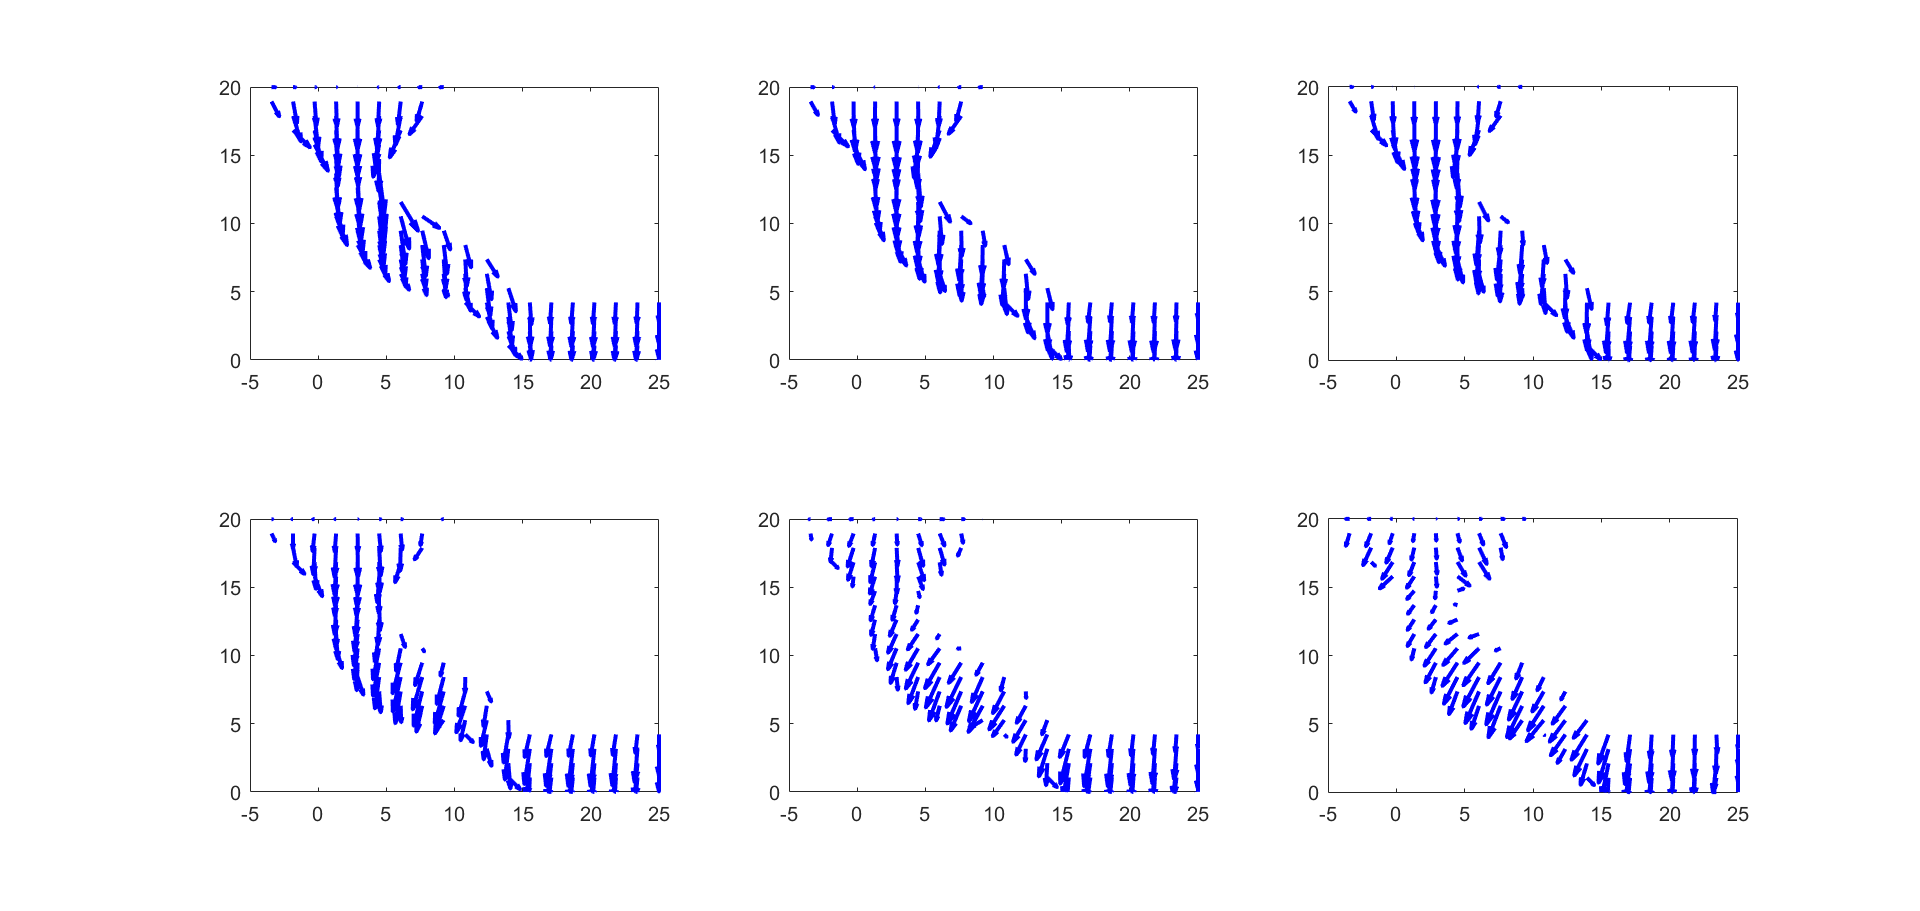
\includegraphics[scale=0.35]{MultiCont2.png}
	\caption{Multishape Example 2: Optimal control} 
	\label{FM2a}
\end{figure}
\\
\\
+++++++++++ I think this is time independent!! ++++++++++++++++++++++++++++
For a third example, we choose a multishape with an imposed background flow and gravity as a target, see Figure \ref{FM3}. The optimal control problem has the same strength of gravity $c = 0.1$ imposed, but no flow. We expect the control to act similar to the flow profile imposed to produce $\hr$. We choose $T = 10$ this time.
We get $J_{FW} = 0.0484$ and $J_{Opt} = 0.0258$ and the results are displayed in Figures \ref{FM3a} and \ref{FM3b}. Furthermore, we compare the strength of $\w$ of the target and the optimal control. The absolute $L_2$/ $L_\infty$ norms are compared, and we get $||\w_{\hr}|| = 68$ and $||\w_{Opt}|| = 50.8965$.
\begin{figure}[h]
	\centering
	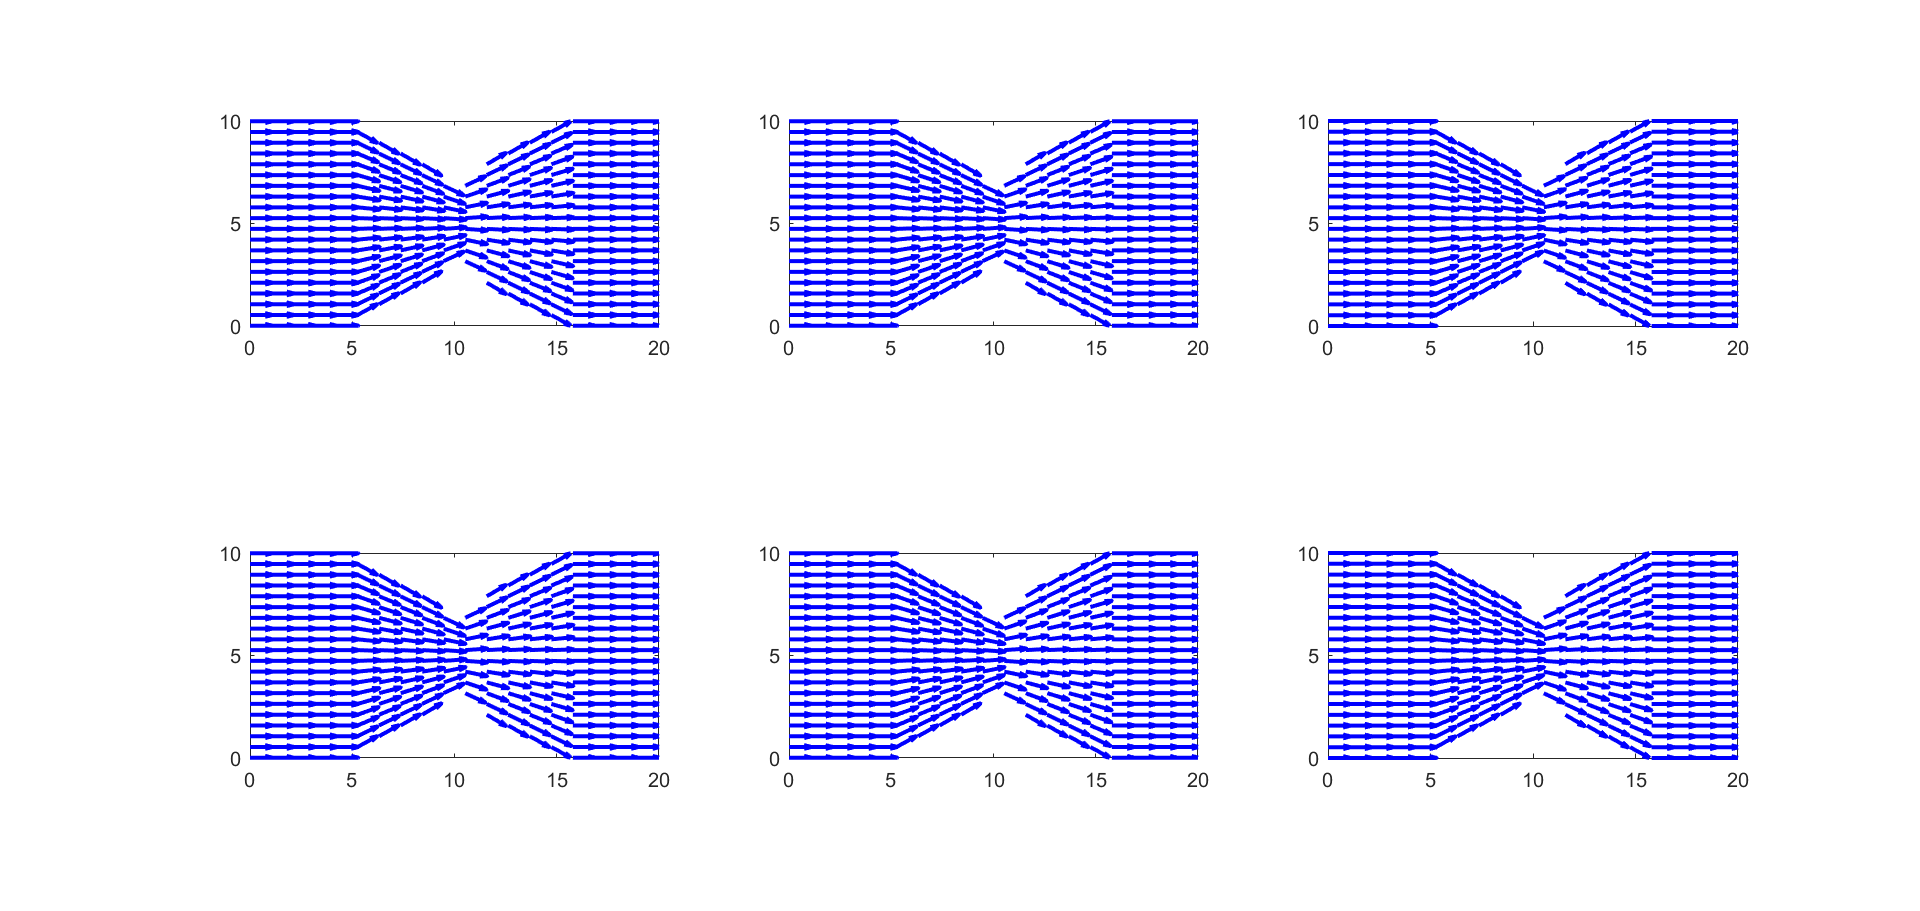
\includegraphics[scale=0.35]{MultiwFW.png}
	\caption{Multishape Example 3:Flow profile determining $\hr$} 
	\label{FM3}
\end{figure}
\begin{figure}[h]
	\centering
	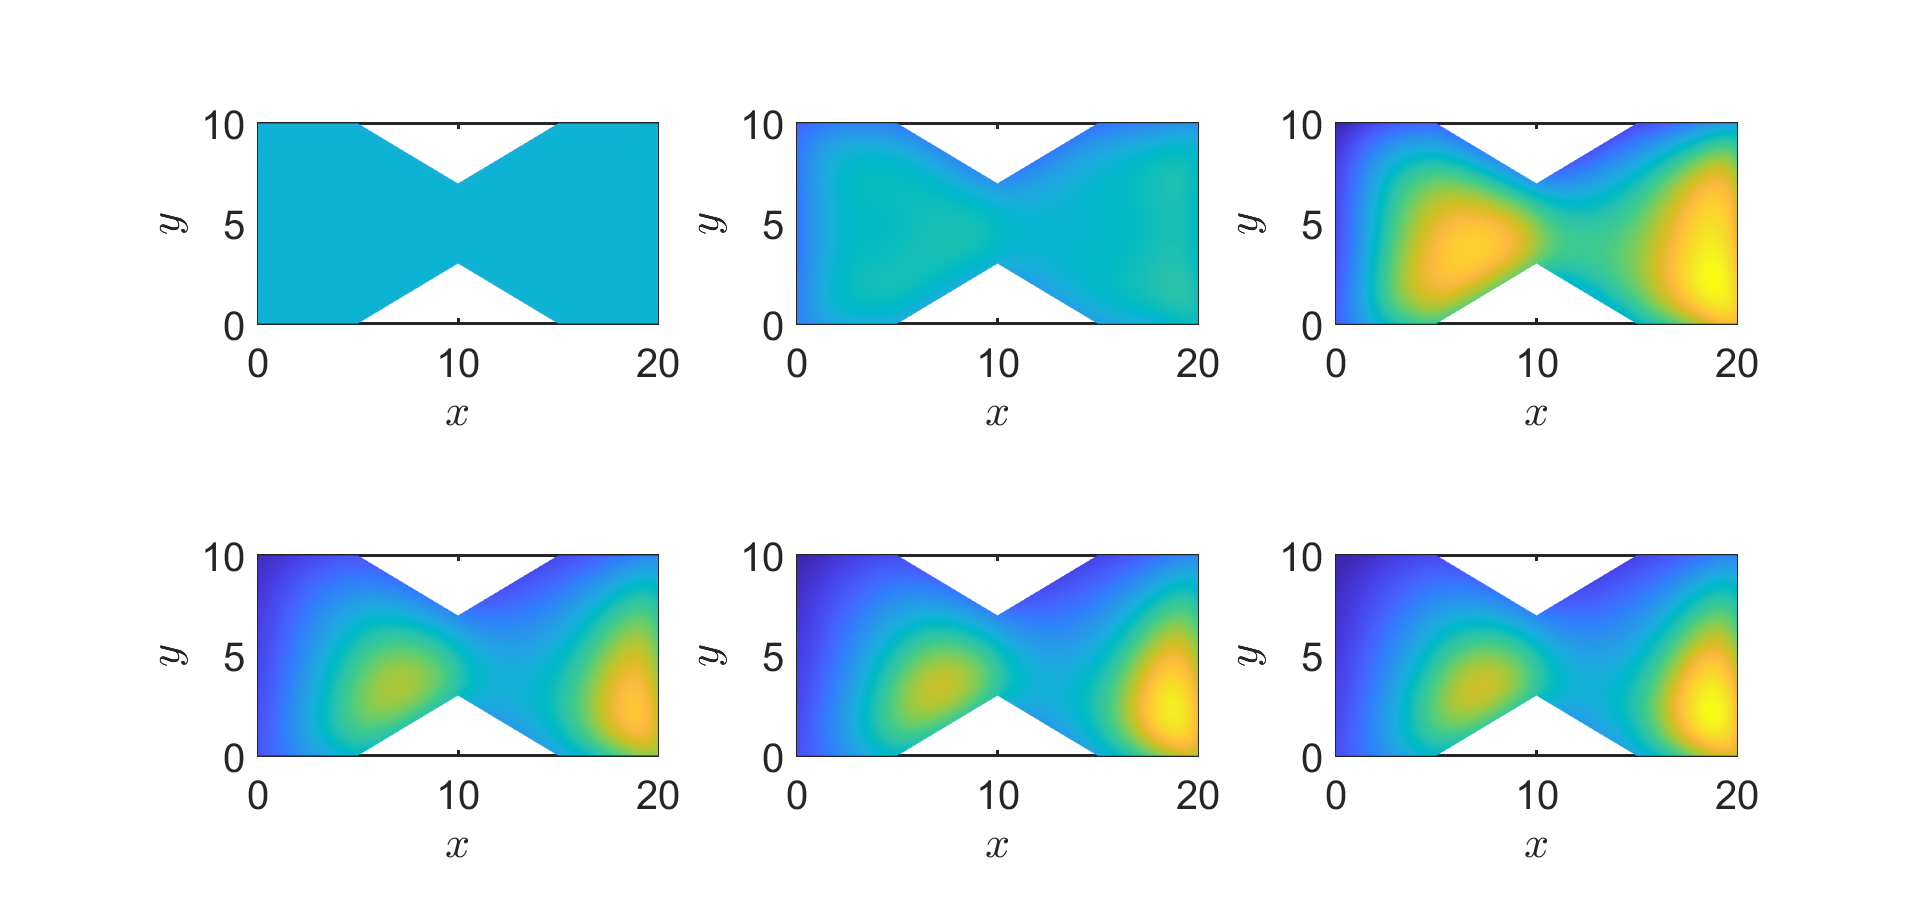
\includegraphics[scale=0.35]{MultiOpt3.png}
	\caption{Multishape Example 3: Optimal $\rho$} 
	\label{FM3a}
\end{figure}
\begin{figure}[h]
	\centering
	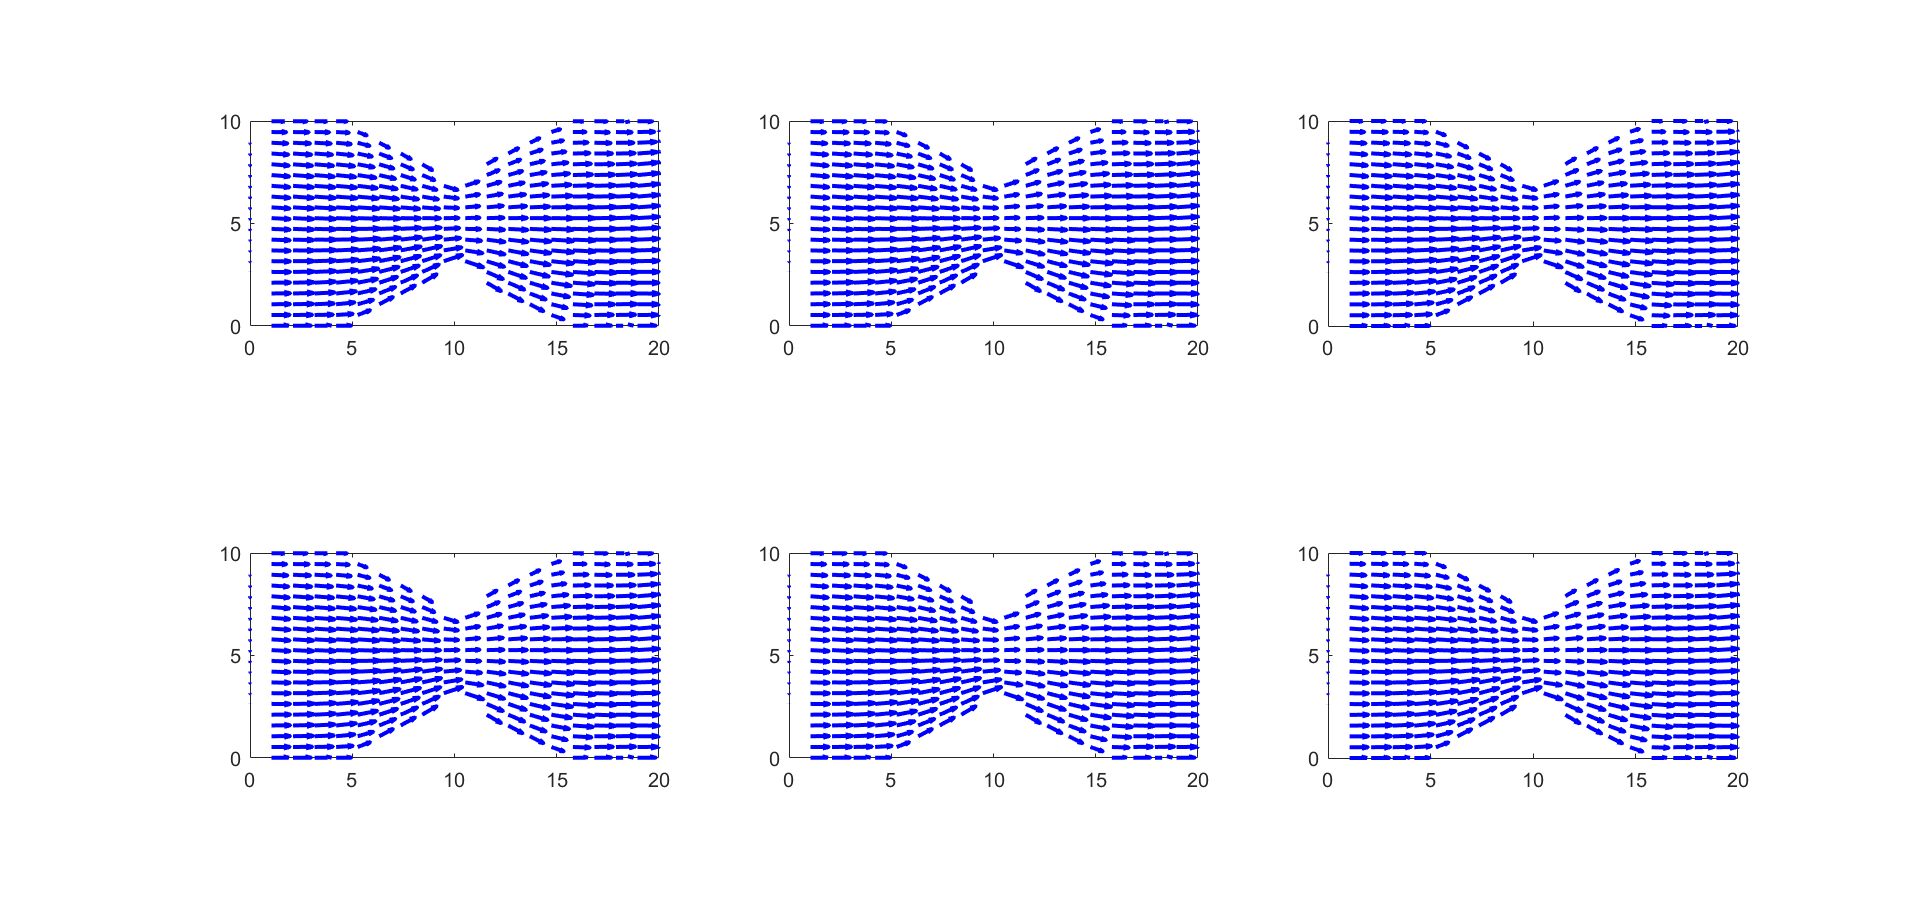
\includegraphics[scale=0.35]{MultiCont3.png}
	\caption{Multishape Example 3: Optimal control} 
	\label{FM3b}
\end{figure}
\subsubsection{Optimization in a Multishape - Time-Independent Control}
We use the first multishape example from the previous section with two quadrilaterals with the same setup and parameter choice. Here, since this is a more difficult problem, we choose $\lambda = 0.001$, which takes considerably more iterations than problems with larger $\lambda$.
We get $J_{FW} = 0.0713$ and $J_{Opt} = 0.0081$ and the result can be seen in Figures \ref{FM1} and \ref{FM2}. If we compare with the time dependent case, as expected for the time independent control, the optimal cost is higher.



\begin{figure}[h]
	\centering
	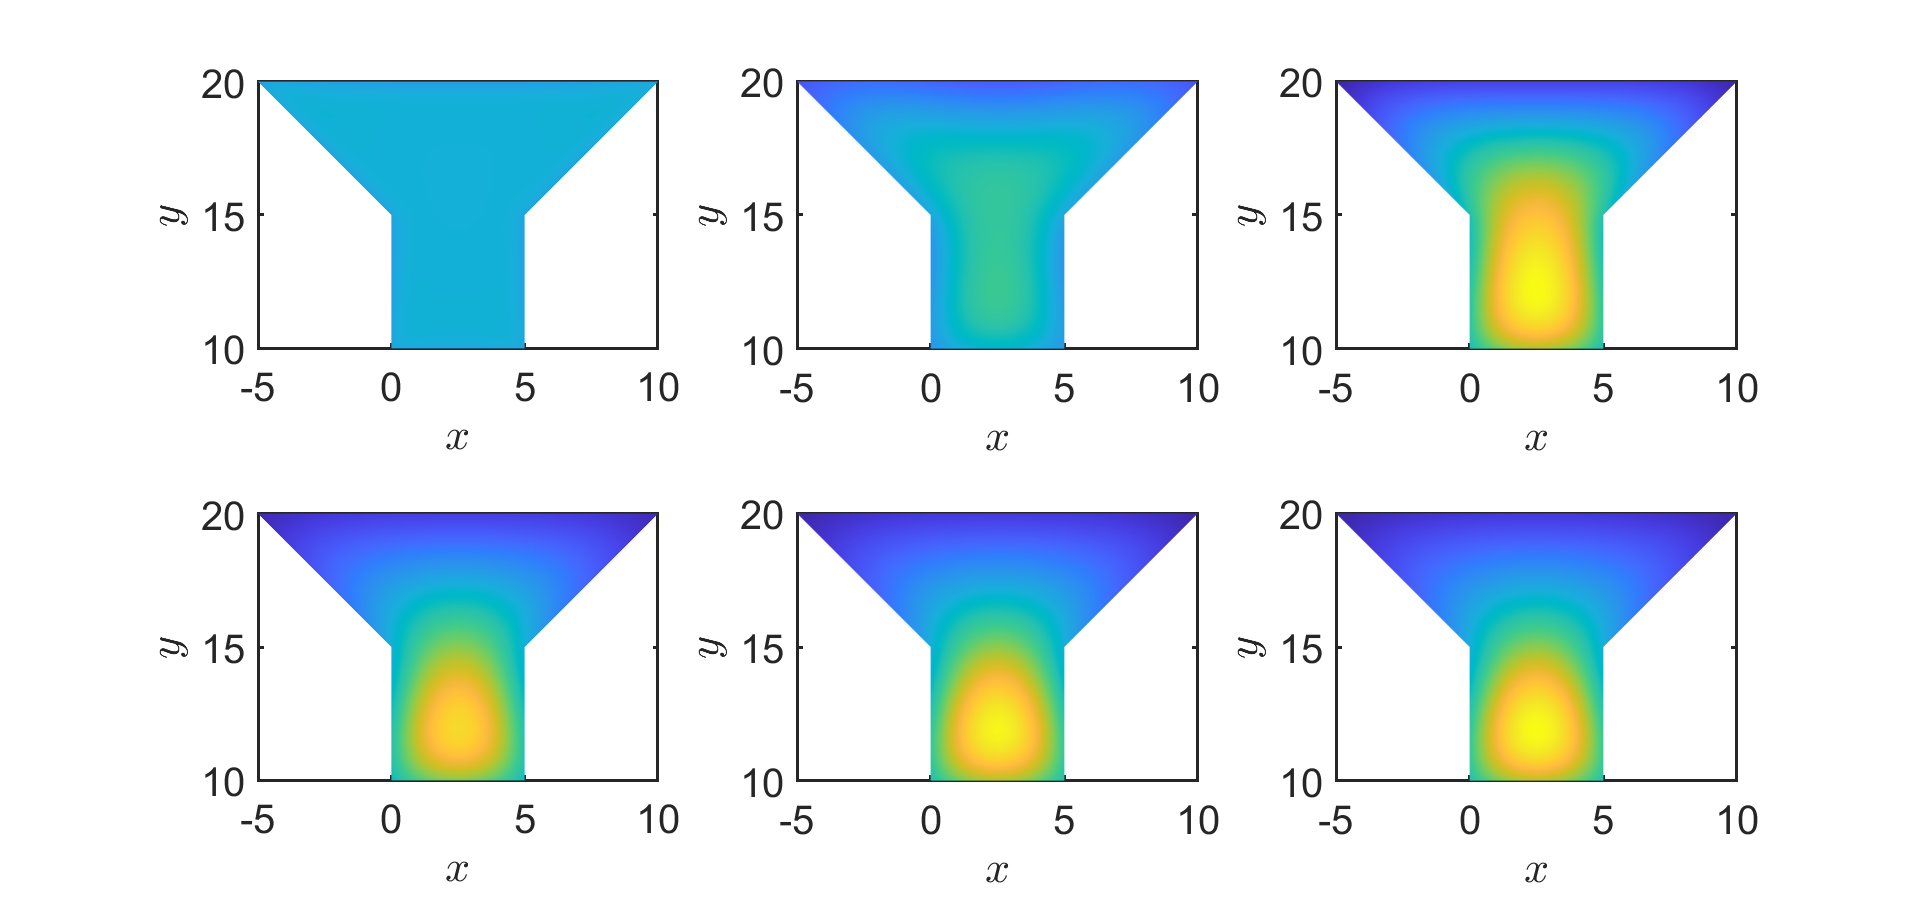
\includegraphics[scale=0.35]{MultiOpt1.png}
	\caption{Multishape Example 1 (time independent control): Optimal $\rho$} 
	\label{FM1}
\end{figure}
\begin{figure}[h]
	\centering
	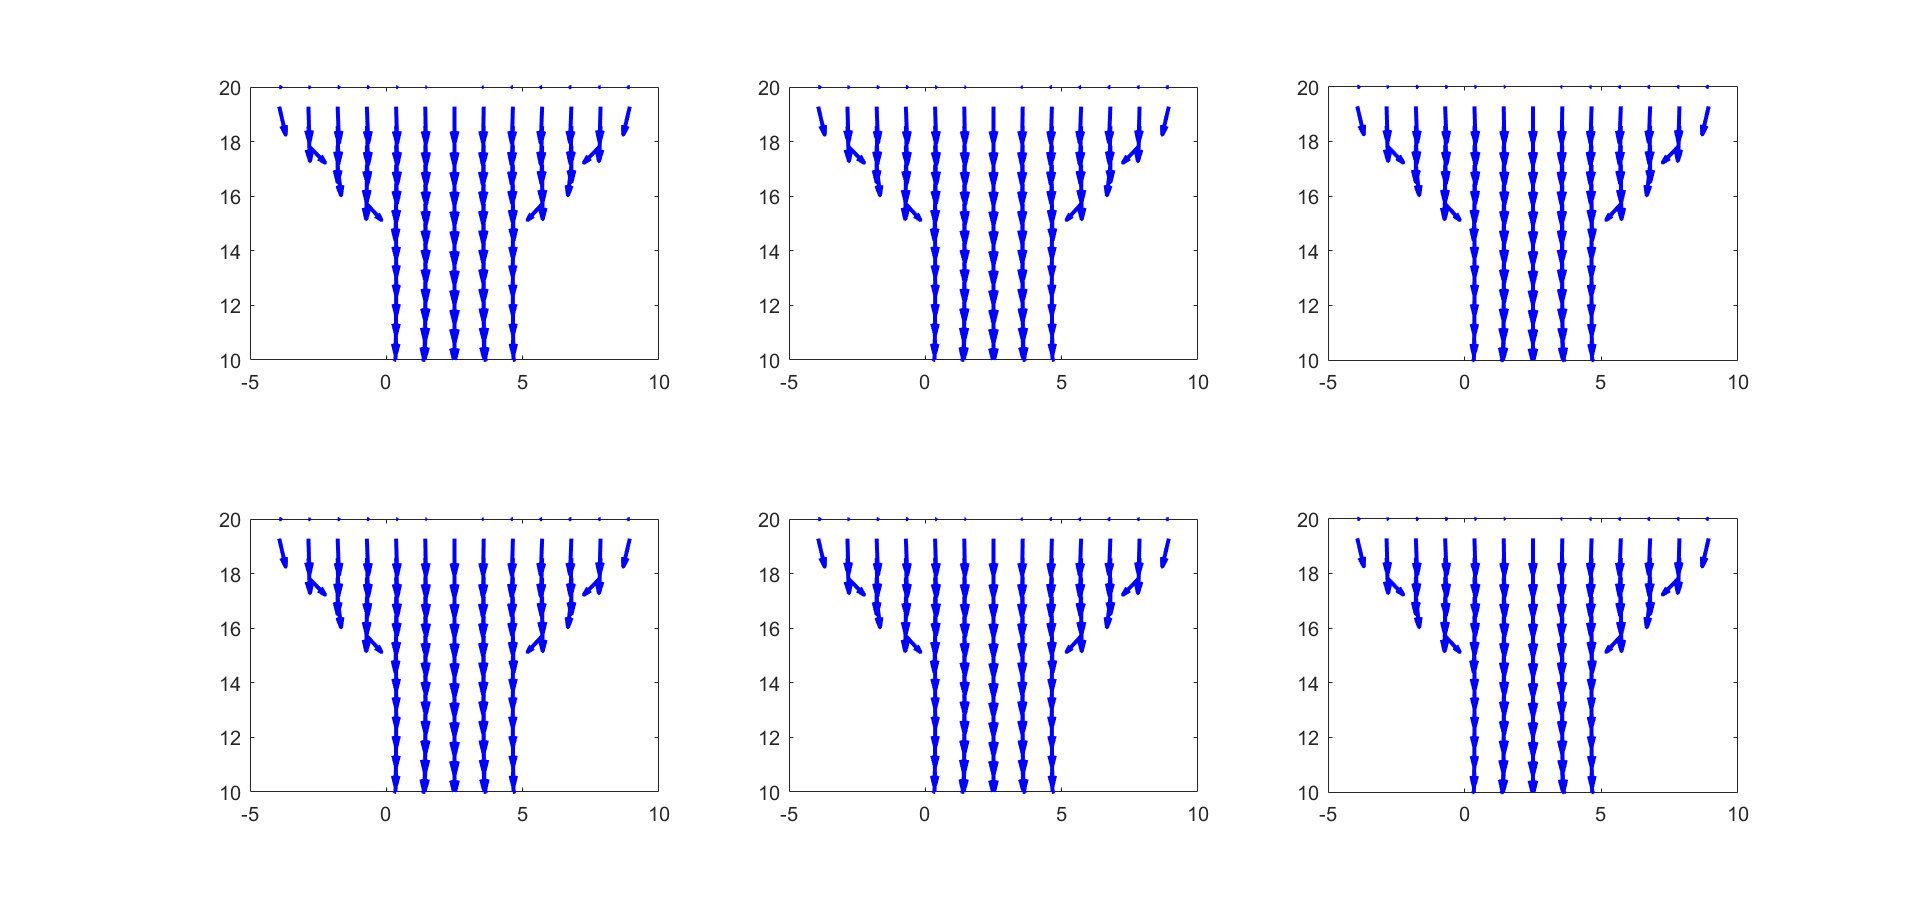
\includegraphics[scale=0.35]{MultiCont1.png}
	\caption{Multishape Example 1 (time independent control): Optimal control} 
	\label{FM2}
\end{figure}

